\section*{1}
Consider the following linear program:\\
maximize $2x_1+ 6x_2$\\
subject to:

$4x_1+x_2 \leq 8$

$x_1+ 2x_2 \leq 6$

$x_1,x_2 \geq 0$\\\\
(a) Draw the feasible solution space on $x_1,x_2$ plane.\\
(b) Give all the vertices of the feasible solution space.\\
(c) What is the optimal value of the objective function?\\
(d) Give the dual of the above primal problem.\\
(e) Draw the feasible solution space for the dual version.\\
(f) What is the optimal solution of the dual version of the problem?
\probLine

\noindent(a)

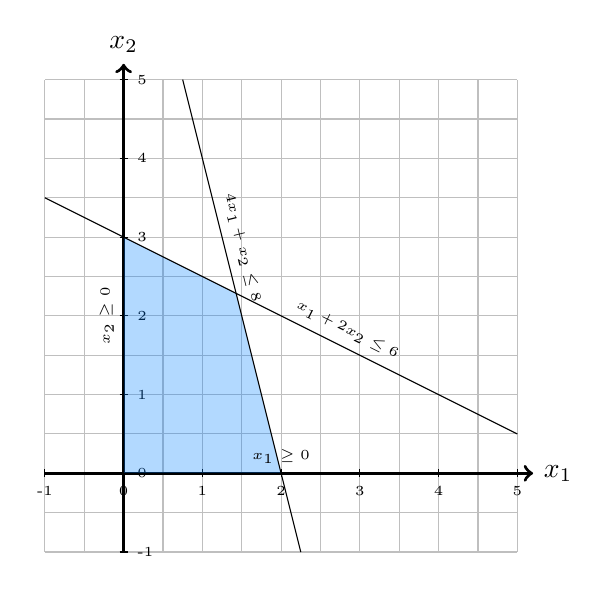
\begin{tikzpicture}

    \draw[gray!50, thin, step=0.5] (-1,-1) grid (5,5);
    \draw[very thick,->] (-1,0) -- (5.2,0) node[right] {$x_1$};
    \draw[very thick,->] (0,-1) -- (0,5.2) node[above] {$x_2$};

    \foreach \x in {-1,...,5} \draw (\x,0.05) -- (\x,-0.05) node[below] {\tiny\x};
    \foreach \y in {-1,...,5} \draw (-0.05,\y) -- (0.05,\y) node[right] {\tiny\y};

    \fill[blue!50!cyan,opacity=0.3] (0,0) -- (0,3) -- (1.4286,2.2857) -- (2,0) -- cycle;

    \draw (0.75,5) -- node[above left,sloped] {\tiny$4x_1+x_2 \leq 8$} (2.25,-1);
    \draw (-1,3.5) -- node[above right,sloped] {\tiny$x_1+2x_2\leq6$} (5,0.5);
    \draw (-1,0) -- node[above,sloped] {\tiny$x_1\geq0$} (5,0);
    \draw (0,-1) -- node[above,sloped] {\tiny$x_2\geq0$} (0,5);

\end{tikzpicture}

\noindent(b) The vertices of the feasible solution space are: $(0,0), (0,3), (1.4286,2.2857), (2,0)$.

\noindent(c) Optimal value for the objective function is at vertex $(x_1,x_2) = (0,3)$ and value is 18.

\noindent(d) The Dual of the problem is:
\\\\
minimize $8p_1+ 6p_2$
\\
subject to:

$4p_1+p_2 \geq 2$

$p_1+ 2p_2 \geq 6$

$p_1,p_2 \geq 0$\\\\

\pagebreak
\noindent(e) 

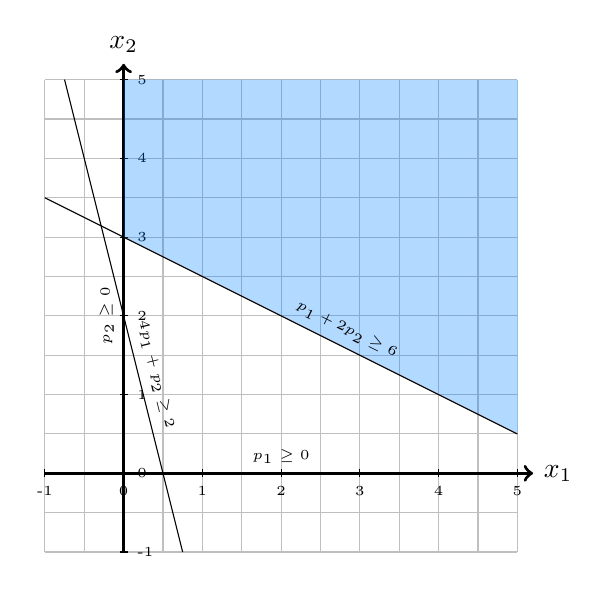
\begin{tikzpicture}

    \draw[gray!50, thin, step=0.5] (-1,-1) grid (5,5);
    \draw[very thick,->] (-1,0) -- (5.2,0) node[right] {$x_1$};
    \draw[very thick,->] (0,-1) -- (0,5.2) node[above] {$x_2$};

    \foreach \x in {-1,...,5} \draw (\x,0.05) -- (\x,-0.05) node[below] {\tiny\x};
    \foreach \y in {-1,...,5} \draw (-0.05,\y) -- (0.05,\y) node[right] {\tiny\y};

    \fill[blue!50!cyan,opacity=0.3] (0,3) -- (0,5) -- (5,5) -- (5,0.5) -- cycle;

    \draw (-0.75,5) -- node[above right,sloped] {\tiny$4p_1+p_2 \geq 2$} (0.75,-1);
    \draw (-1,3.5) -- node[above right,sloped] {\tiny$p_1+2p_2 \geq 6$} (5,0.5);
    \draw (-1,0) -- node[above,sloped] {\tiny$p_1\geq0$} (5,0);
    \draw (0,-1) -- node[above,sloped] {\tiny$p_2\geq0$} (0,5);

\end{tikzpicture}

(f) Optimal value for the objective function of the dual is at vertex $(x_1,x_2) = (0,3)$ and value is 18.

